\chapter{THE ODOO SOFTWARE} 
\pagenumbering{arabic} %設定頁號阿拉伯數字
\setcounter{page}{26}  %設定頁數
\begin{center}
\fontsize{18}{16}\selectfont \textbf{ODOO 軟體}\\
\end{center}


\section{Introduction to the Odoo software ODOO軟體簡介}
\fontsize{12}{2.5pt}\sectionef  
{Odoo is a commercial business management software with strong ties to the open source community. Initially started as open source ERP software becoming well received as an affordable and intuitive package that thrived on integration and expandability. Since then, as the company experienced accelerated growth, it shifted their business model to include an enterprise paid version as well as an online service.}\\[1pt]

\fontsize{12}{2.5pt}\sectionef 
{本論文的目的是透過分析包含所述整合的不同概念和動態,找出使用現成的 Odoo 軟體可以實現 PLM+MES 系統的程度,並應用一個虛構的場景來確定這些概念是否以及哪些概念包含在此打包解決方案中。}\\[15pt]

\fontsize{12}{2.5pt}\sectionef
{To contextualize, the Odoo software differs from other solutions in the market substantially both in implementation and business model. To summarize, the Odoo software 
was originated as an open-source ERP software as oppose to a PLM or MES software and as such its availability and modularity are reasonably expanded. It goes without saying that the counter point for this that its usability in the field of PLM or MES is uncertain hence the value of this work.}\\[1pt]

\fontsize{12}{2.5pt}\sectionef  
{如同 2.2 節中所提到的,現代 ERP 系統通常是模組化的,並且在以 Odoo 為例,由於數量驚人,這種模組化尤為明顯
由社區開發的模組以及公司開發的模組提供的擴展模組高度整合。 這種可擴展性使得該軟體如此重要回到 PLM+MES 整合的主題,因為現有的 PLM 模組以及其製造模組中具有顯著的 MES 功能。}\\[15pt]

\fontsize{12}{2.5pt}\sectionef  
{Within the scope of this thesis, the objective is to utilize this software on the management of the previously mentioned fictional company and draw conclusions regarding how effective the integration of PLM and MES is already present within this system.  }\\[1pt]

\fontsize{12}{2.5pt}\sectionef 
{在本論文的範圍內,目標是利用該軟體進行管理前面提到的虛構公司,並就其有效性得出結論PLM 和 MES 的整合已經存在於該系統中。}\\[15pt]

\section{How it works 如何運作 }
\fontsize{12}{2.5pt}\sectionef 
 {The software can be installed in most x86 computers and it supports several operating
systems including windows and all the main Linux distributions.}\\[1pt]

\fontsize{12}{2.5pt}\sectionef  
{該軟體可以安裝在大多數x86電腦上,並且支援多種操作
系統包括 Windows 和所有主要的 Linux 發行版。}\\[15pt]

\fontsize{12}{2.5pt}\sectionef 
 {Ideally, the Odoo software is installed in a computer connected to a local area networkand starts a SQLdatabase that holds all the necessary information and files produced by thebusiness (Figure 16). Said computer works essentially as a server and accessed via abrowser by the other machines present in the network. This computer can be a dedicatedserver or a working desktop in use, but it is important to remember that it must remain ONand connected throughout the entire time the software is required to function.}\\[1pt]

\fontsize{12}{2.5pt}\sectionef  
{理想情況下,Odoo 軟體安裝在連接到區域網路的電腦上並啟動一個 SQL 資料庫,其中包含由該程式產生的所有必要資訊和文件業務(圖 16)。 所述計算機本質上作為伺服器工作並透過網路中其他機器的瀏覽器。 這台計算機可以是專用的伺服器或正在使用的工作桌面,但重要的是要記住它必須保持開啟狀態並且在軟體需要運作的整個過程中都保持連線。}
\\[15pt]


\begin{figure}[hbt!]
\begin{center}
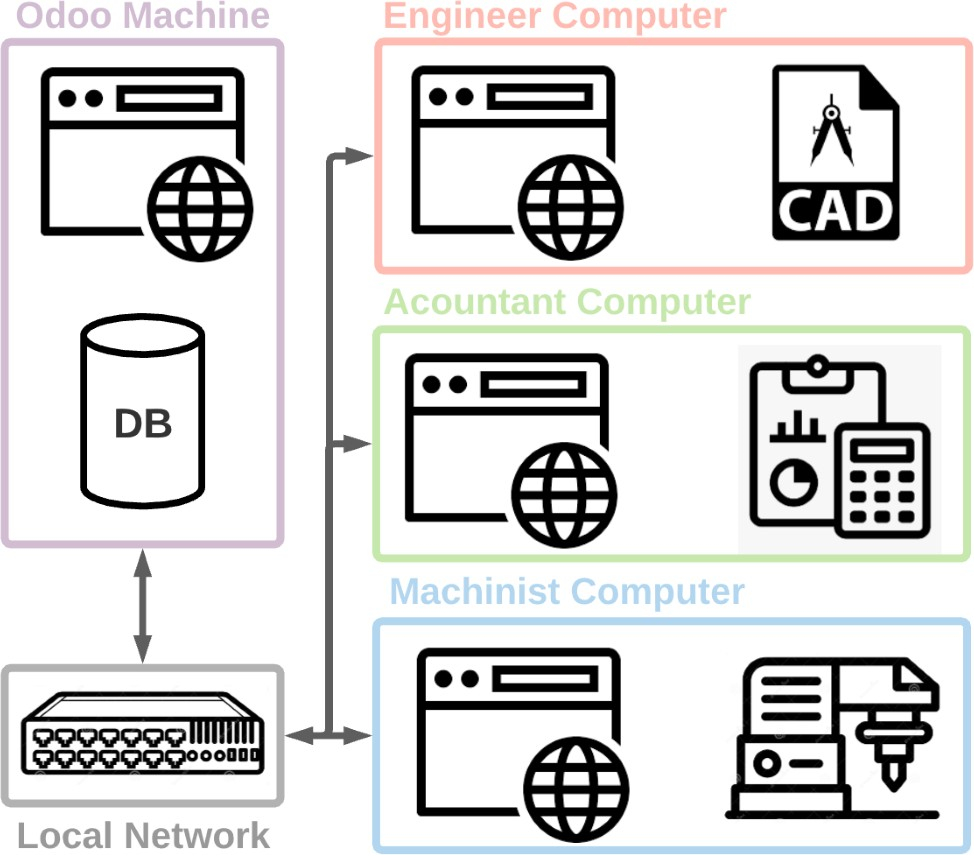
\includegraphics[width=15cm]{16}
\caption{\Large  Function Diagram of Odoo configuration A Odoo配置A功能圖}\label{fig.16}
\end{center}
\end{figure}


\fontsize{12}{2.5pt}\sectionef 
 {Another option is to use the hosting service provided by Odoo SA (Figure 17). In this case
the system would be hosted by them and data would be stored in their cloud. This is a good
fit for many small businesses specially if they are particularly fond of the website related
modules (used to build and manage web sites and e-stores). It is however network dependent
which may pose a problem in some instances.}\\[1pt]

\fontsize{12}{2.5pt}\sectionef  
{另一個選擇是使用 Odoo SA 提供的託管服務(圖 17)。 在這種情況下
該系統將由他們託管,數據將儲存在他們的雲端中。 這是一個很好的
適合許多小型企業,特別是如果他們特別喜歡相關網站
模組(用於建立和管理網站和電子商店)。 然而,它依賴於網絡
這在某些情況下可能會造成問題。}
\\[15pt]


\begin{figure}[hbt!]
\begin{center}
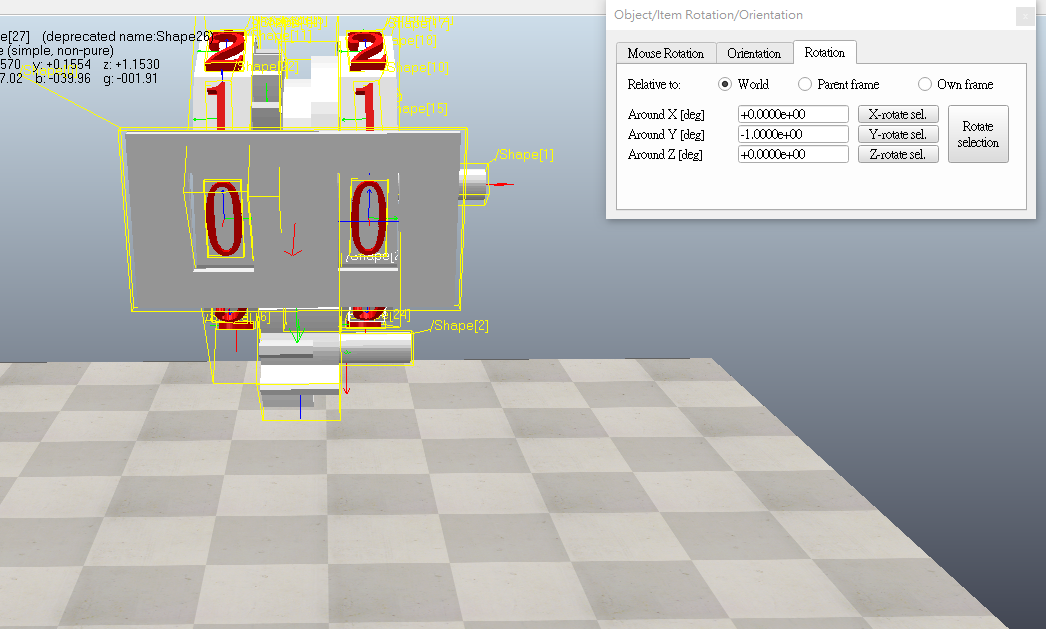
\includegraphics[width=15cm]{17}
\caption{\Large  Function Diagram of Odoo configuration B Odoo配置B功能圖}\label{fig.17}
\end{center}
\end{figure}

\fontsize{12}{2.5pt}\sectionef 
 {Users essentially interact with the system through the graphical user interface (GUI) and
use it to access the different modules available as need by a per user basis. This means that
restrictions can be applied to different users in order to maintain control over the different
aspects of the business activity, e.g., accountants would get access to accounting module,
sales module and inventory module but they would be restricted from the manufacturing
module. This sort of restriction guarantees control over the processes only to the proper
employees.}\\[1pt]

\fontsize{12}{2.5pt}\sectionef  
{使用者本質上是透過圖形使用者介面(GUI)與系統互動的使用它可以根據每個用戶的需要存取可用的不同模組。 這意味著可以對不同的使用者套用限制,以維持對不同使用者的控制業務活動的各個方面,例如會計師可以存取會計模組,銷售模組和庫存模組,但它們將被限制在製造中模組。 這種限制保證了只有適當的人才能控制流程僱員。}
\\[15pt]


\fontsize{12}{2.5pt}\sectionef 
 {Within said GUI the different modules appear as app icons (Figure 18) and, from the getgo, the company has available a reasonable selection of well-integrated applications not to mention a vast app store filled with community made modules.}\\[1pt]

\fontsize{12}{2.5pt}\sectionef  
{在所述GUI 中,不同的模組顯示為應用程式圖標(圖18),並且從一開始,該公司就提供了合理的整合良好的應用程式選擇,更不用說充滿社區製作模組的龐大應用程式商店。}
\\[15pt]


\begin{figure}[hbt!]
\begin{center}
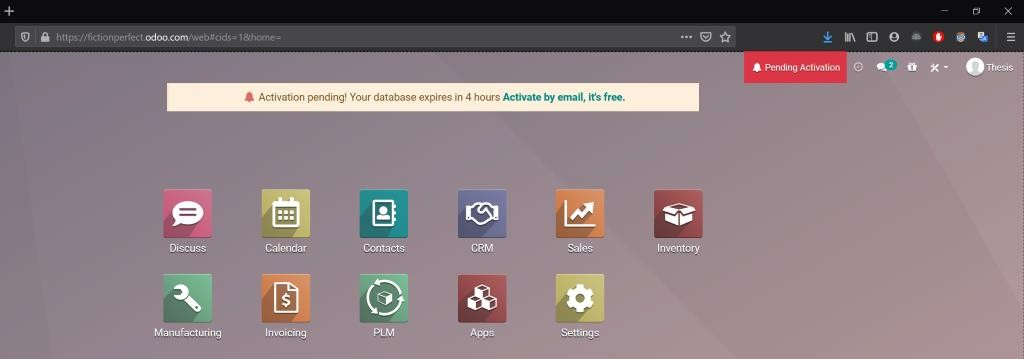
\includegraphics[width=15cm]{18}
\caption{\Large Screenshot of GUI from Odoo in configuration B 配置 B 中 Odoo 的 GUI 螢幕截圖}\label{fig.18}
\end{center}
\end{figure}

\section{Odoo’s view on manufacturing: Odoo 對製造業的看法:}


\fontsize{12}{2.5pt}\sectionef 
 {Odoo considers that the responsibilities regarding manufacturing of anything is distributed throughout different company departments, each of which is responsible for
specific file types and dealt with using specific apps (Table 2). From the perspective of PLM this is very positive because as mentioned by (Saaksvuori and Immonen, 2008) about User privilege management – the PLM system is used to define information access and maintenance rights. The PLM system defines the people who can create new information or make, check and accept changes, and those who are allowed only to view the information or documents in the system. user privilege management is usually a challenge when regardingintegration of PLM with other systems.}\\[1pt]

\fontsize{12}{2.5pt}\sectionef  
{Odoo 認為任何產品製造的責任都是分佈在公司不同部門,各部門負責特定的文件類型並使用特定的應用程式進行處理(表 2)。 從PLM的角度來看這是非常正面的,因為正如(Saaksvuori 和 Immonen,2008)關於使用者所提到的權限管理-PLM系統用於定義資訊存取和維護權利。 PLM 系統定義了可以建立新資訊或進行、檢查和接受更改,以及那些僅被允許查看資訊或系統中的文件。 使用者權限管理通常是一個挑戰PLM 與其他系統的整合。}
\\[15pt]


\begin{table}[htbp]
    \centering
    \begin{tabular}{|c|c|}
        \hline
         Department 部門& Documents/Apps 文件/應用程式\\
        \hline
        Engineering  工程& CAD BOM CAD 和物料清單 \\
        Manufacturing Engineering  製造工程& Routings, Worksheets, Workcenters 工藝路線、工作表、工作中心\\
       Purchase/Procurement 採購/採購& Procurement order, Request for quotation 採購訂單、詢價單\\
       Inventory Operators 庫存操作員&Receipt, Barcode 收據、條碼 \\
       Manufacturing Foreman 製造工長& Manufacturing order, Planning 製造訂單、計劃 \\
       Manufacturing Operators 製造經營者& Work order工作指示 \\
       Inventory Operators 庫存操作員& Delivery送貨 \\
       Quality 品質& Alert, Analysis, Control points 警報、分析、控制點\\、
      Engineering  工程& Engineering change order工程變更單 \\
      Maintenance 維護& Preventive/Corrective 預防/糾正\\
        \hline
    \end{tabular}
\end{table}


\fontsize{12}{2.5pt}\sectionef 
 {From Odoo’s perspective in the beginning of any usual manufacturing process, the first
step will be the engineers designing the product usually using a CAD software. Once that is
done, they will create a Bill of materials (BOM) this is a list of components or materials
necessary to produce the product. At this point the focus goes to the manufacturing process
itself.}\\[1pt]

\fontsize{12}{2.5pt}\sectionef  
{從 Odoo 的角度來看,在任何通常的製造過程開始時,第一個
步驟是工程師通常使用 CAD 軟體設計產品。 一旦那是
完成後,他們將創建物料清單 (BOM),這是組件或材料的列表
生產產品所必需的。 此時重點轉向製造過程
本身。}
\\[15pt]

\fontsize{12}{2.5pt}\sectionef 
 {The software view of process is focused on routings, worksheets and work centers this is
done by the manufacturing engineering team. A routing is a set of steps a product goes
through for production. Worksheets are the instructions for the manufacturing operator, and
work centers are the places where the production is being conducted. Odoo considers that
these are the requirements for putting engineers plans in motion}\\[1pt]

\fontsize{12}{2.5pt}\sectionef  
{流程的軟體視圖側重於工藝路線、工作表和工作中心,這是
由製造工程團隊完成。 製程路線是產品運作的一組步驟
透過進行生產。 工作表是給製造操作員的說明,並且
工作中心是進行生產的地方。 奧杜認為
這些是實施工程師計劃的要求}
\\[15pt]

\fontsize{12}{2.5pt}\sectionef 
 {A procurement department will be responsible for requesting for quotations (RFQ) or
purchase orders (PO). Inventory operators take care of receipts based on those POs, which is
usually done using a barcode application within Odoo. As explained in the first section of
this chapter Odoo is primarily an ERP system and it is at this point that it is possible to notice
some ERP centric characteristics like the focus on inventory and management of resources.
This will be further analyzed in the following sections, but it is fair to point out that those
RFQ and PO are considered items within the data base.}\\[1pt]

\fontsize{12}{2.5pt}\sectionef  
{採購部門將負責索取報價(RFQ)或
採購訂單 (PO)。 庫存操作員根據這些 PO 處理收貨,即
通常使用 Odoo 中的條碼應用程式完成。 正如第一節所解釋的
本章 Odoo 主要是一個 ERP 系統,此時可以注意到
一些以 ERP 為中心的特徵,例如專注於庫存和資源管理。
這將在以下各節中進一步分析,但公平地指出,這些
RFQ 和 PO 被視為資料庫中的項目。}
\\[15pt]

\fontsize{12}{2.5pt}\sectionef 
 {Only when you have the design the process and the materials required Odoo considers
manufacturing possible. Then the manufacturing foreman will create a manufacturing order
(MO) and manage the planning of the manufacturing operators through work orders (WO)
and work centers. Then the manufacturing operators can start production following a work
order. After the products are produced, they automatically appear in the inventory database
which alongside packaging and delivery is managed by the Inventory department.}\\[1pt]

\fontsize{12}{2.5pt}\sectionef  
{只有當您設計了 Odoo 考慮的流程和所需材料時
製造成為可能。 然後製造工長將創建製造訂單
(MO) 並透過工單管理製造操作員的計畫 (WO)
和工作中心。 然後製造操作員可以在工作結束後開始生產
命令。 產品生產出來後,自動出現在庫存資料庫中
與包裝和交付一起由庫存部門管理。}
\\[15pt]


\fontsize{12}{2.5pt}\sectionef 
 {Odoo considers that quality team is responsible for assign control/check points as well as
identify possible issues within the product or production. These quality control check points
are very interesting from the MES perspective because it represents valuable production data
that is collected in real time as production occurs, i.e., it is possible to assign a dimension
check after the production of every piece where the machinist will fill in the dimensions to
track quality over time.}\\[1pt]

\fontsize{12}{2.5pt}\sectionef  
{Odoo 認為品質團隊負責分配控制/檢查點以及
識別產品或生產中可能存在的問題。 這些品質控制檢查點
從 MES 的角度來看非常有趣,因為它代表了有價值的生產數據
在生產發生時即時收集,即可以分配維度
每件產品生產完成後進行檢查,機械師將填寫尺寸
隨著時間的推移跟踪品質。}
\\[15pt]


\fontsize{12}{2.5pt}\sectionef 
 {If it's a problem of design or if there is possibility for improvement an engineering change
order (ECO) can be issued. This falls back to the hands of the manufacturing engineering
team and will focus on updating documents and the BOM. The ECO is the heart of how Odoo
deals with tracking change within the system. That is key when regarding PLM and in fact is
the focus of the Odoo application called PLM. To which lengths said application is capable
to perform is the subject of the next section.}\\[1pt]

\fontsize{12}{2.5pt}\sectionef  
{如果是設計問題或是否有改進工程變更的可能性
可以發出訂單(ECO)。 這又回到了製造工程的手中
團隊將專注於更新文件和 BOM。 ECO 是 Odoo 的核心
處理追蹤系統內的變化。 對於 PLM 而言,這是關鍵,事實上
Odoo 應用程式的焦點稱為 PLM。 所述應用程式能夠達到什麼長度
執行是下一節的主題。}
\\[15pt]

\section{The information structure of Odoo Odoo的資訊結構 }

\fontsize{12}{2.5pt}\sectionef 
 {Each module focuses in the manipulation of specific object-oriented classes that hold
metadata within the database. These are the virtual Items that are responsible for virtualizing
the aspects of the product lifecycle as referred by in (Section 3.1). Different types of items
have different types of accounts and hold different sorts of data, i.e., a product item is
representative of a certain product and holds metadata that is relevant to its interactions and
use as well as links to other possible items that are closely relevant like their responsible user
or the bill of materials necessary to its manufacturing. Odoo them makes all that information
accessible and interactable through its browser interface (Figure 19 and Figure 20). For the
sake of consistency this document will refer to specific item representations (E.g. Bolt) as
‘item’ and refer to a type of item (Product) as ‘item class’.}\\[1pt]

\fontsize{12}{2.5pt}\sectionef  
{每個模組都專注於特定物件導向類別的操作,這些類別包含
資料庫內的元資料。 這些都是負責虛擬化的虛擬項
(第 3.1 節)中提到的產品生命週期的各個面向。 不同類型的物品
擁有不同類型的帳戶並保存不同類型的數據,即產品項目是
代表某個產品並保存與其互動相關的元數據
使用以及指向其他可能的項目的鏈接,這些項目與其負責的用戶密切相關
或其製造所需的物料清單。 Odoo 他們製作了所有這些資訊
可透過其瀏覽器介面進行存取和互動(圖 19 和圖 20)。 為了
為了保持一致性,本文檔將特定的項目表示(例如螺栓)稱為
「item」並將某種類型的項目(產品)稱為「項目類別」。}\\[15pt]

\begin{figure}[hbt!]
\begin{center}
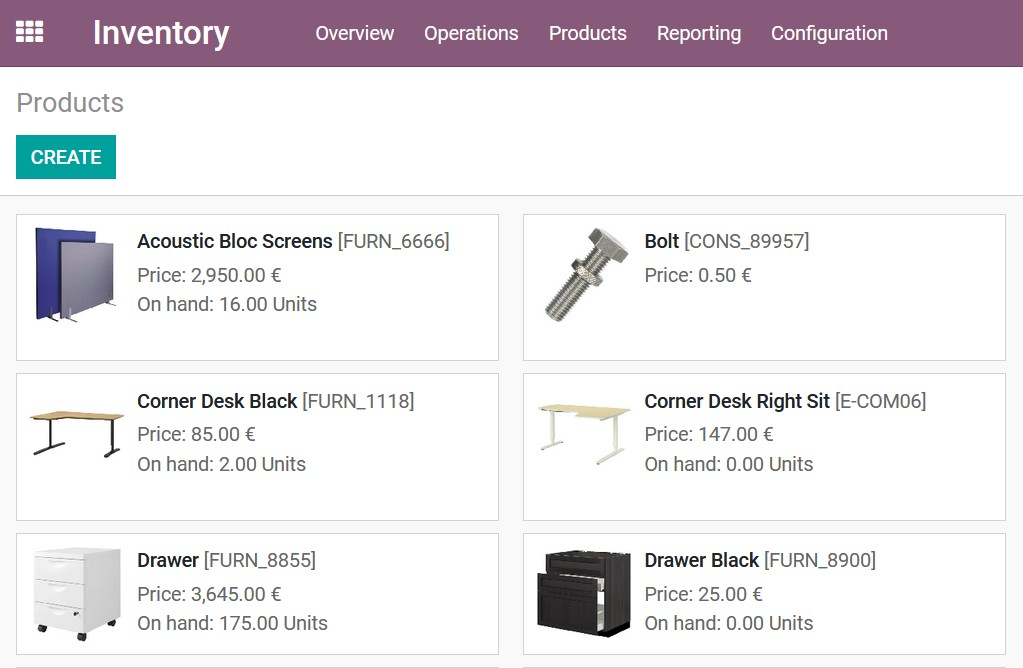
\includegraphics[width=15cm]{19}
\caption{\Large Example of Odoo’s interface regarding items Odoo 有關專案的介面範例}\label{fig.19}
\end{center}
\end{figure}

\begin{figure}[hbt!]
\begin{center}
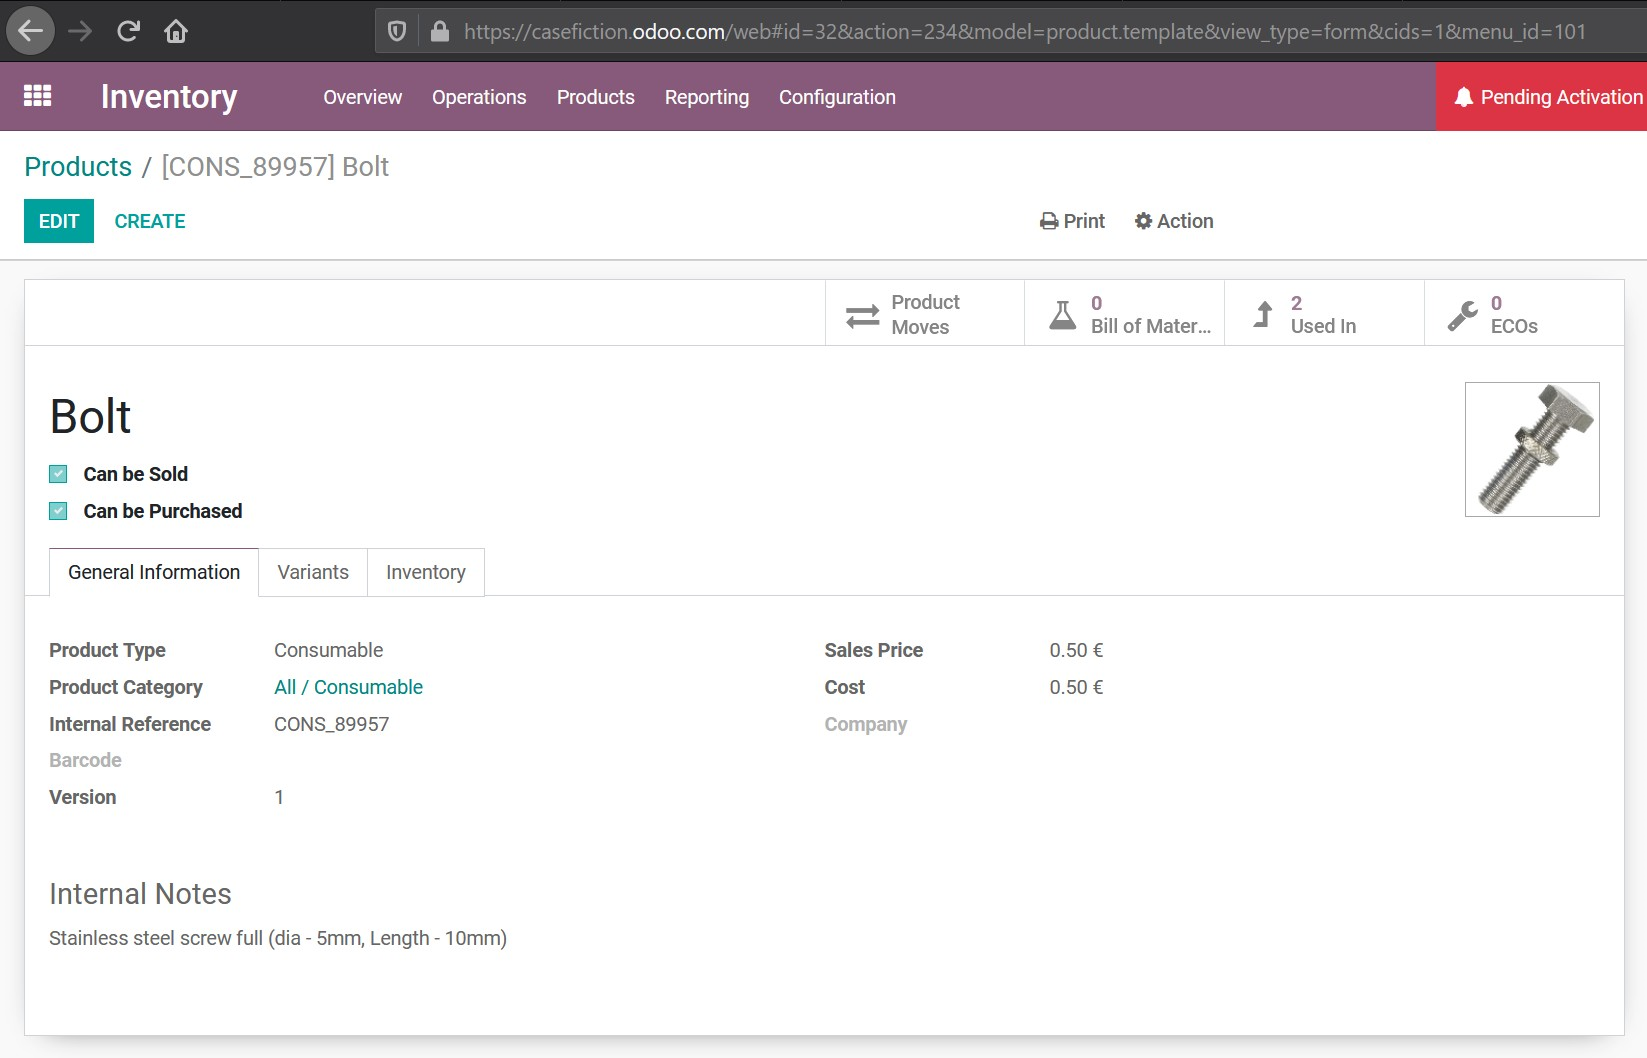
\includegraphics[width=15cm]{20}
\caption{\Large Example of specific item and its metadata as displayed by GUI GUI 顯示的特定項目及其元資料的範例}\label{fig.20}
\end{center}
\end{figure}


\fontsize{12}{2.5pt}\sectionef 
 {Within Odoo, there are several types of those item classes (some holding a lot of metadata
and some holding very little) all with a varying degree of relationships and integration. Since
the scope of this work is limited to the PLM and MES capabilities, the focus is on the items
that are related to it. The following sections will provide short explanations for the main 7
item classes of Odoo’s manufacturing process since its basic understanding is helpful for the
reader to follow the simulation. These are represented in the following diagram (Figure 21).
Other items that are external to the manufacturing procedure will be presented throughout
the simulation.}\\[1pt]

\fontsize{12}{2.5pt}\sectionef  
{在 Odoo 中,這些項目類有多種類型(有些包含大量元資料)
有些持有很少),所有這些都具有不同程度的關係和整合。 自從
這項工作的範圍僅限於 PLM 和 MES 功能,重點是專案
與它相關的。 以下部分將對主要 7 個部分進行簡短說明
Odoo 製造流程的專案類別,因為它的基本了解有助於
讀者跟隨模擬。 這些如下圖所示(圖 21)。
製造過程之外的其他項目將在整個過程中呈現
模擬。}\\[15pt]


\begin{figure}[hbt!]
\begin{center}
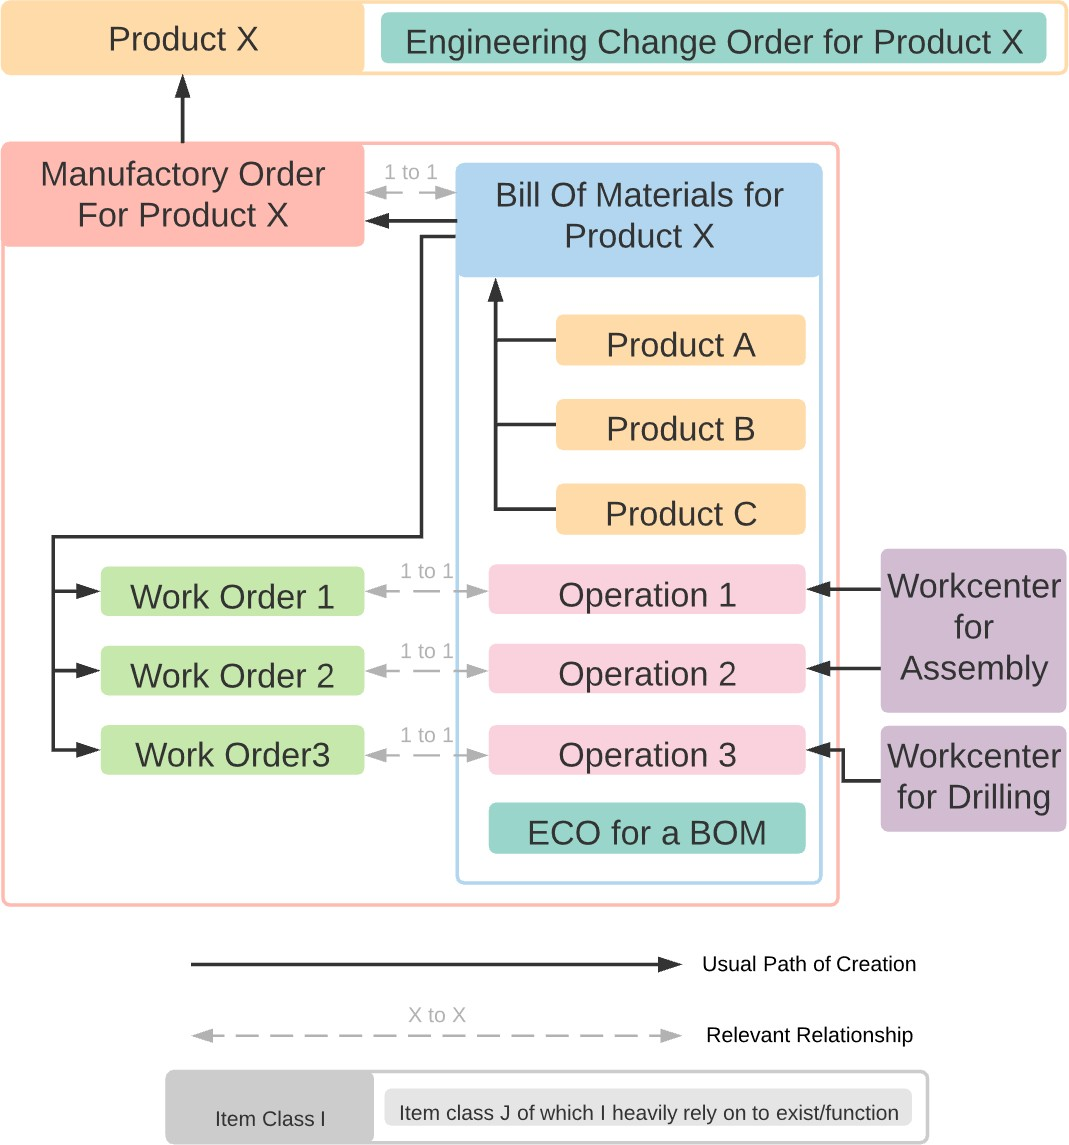
\includegraphics[width=15cm]{21}
\caption{\Large Simplified Item relation diagram to the manufacturing of a product X  與產品 X 的製造相關的簡化專案關係圖}\label{fig.21}
\end{center}
\end{figure}



\section{Product Item 產品項目 }

\fontsize{12}{2.5pt}\sectionef 
 {Every material, component or product is characterized by a PRODUCT type class that is
held and mainly managed within the Inventory application of Odoo. That means that within
the system product production is dependent on the availability of other products that are
either bought as they are or manufactured from another products (Figure 22), i.e., raw
materials are considered products as well, more specifically products that are purchased and
then included in the BOM’s to manufacture other products. This is considered the main item
class since it is both the source and the goal of manufacturing.
}\\[1pt]

\fontsize{12}{2.5pt}\sectionef  
{每種材料、組件或產品都具有一個產品類型類別,該類別是
主要在 Odoo 的庫存應用程式中進行持有和管理。 這意味著在
系統產品的生產取決於其他產品的可用性
要麼按原樣購買,要麼用其他產品製造(圖 22),即原料
材料也被視為產品,更具體地說,是購買和使用的產品
然後包含在 BOM 中以製造其他產品。 這被認為是主要項目
階級,因為它既是製造的源泉,也是製造的目標。}\\[15pt]


\begin{figure}[hbt!]
\begin{center}
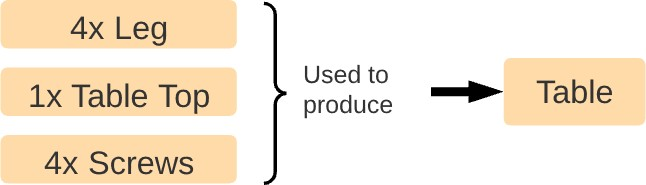
\includegraphics[width=15cm]{22}
\caption{\Large  simplified Product relation diagram  簡化的產品關係圖}\label{fig.22}
\end{center}
\end{figure}


\section{Operation item class and workcenter item class 操作項目類和工作中心項目類}

\fontsize{12}{2.5pt}\sectionef 
 {The operation item is representative of a manufacturing operation that is required to
transform components or raw materials into a product or new component while the
workcenter item represents the place at which the operation takes place, e.g., a sanding wood
will be carried out in a sanding station (Figure 23) that has the proper equipment. The
workcenter is eventually used in Odoo as a time/equipment management tool in its
production planning. Basically, when the production center is at full capacity it puts
following processes on hold or redirects the processes to an alternative workcenter. The
operation item is also responsible for holding the instruction files that are consulted during
production. }\\[1pt]

\fontsize{12}{2.5pt}\sectionef  
{操作項目代表製造操作,需要
將組件或原料轉化為產品或新組件,同時
工作中心項代表進行操作的地點,例如打磨木材
將在具有適當設備的打磨站(圖 23)中進行。 這
workcenter 最終在 Odoo 中用作時間/設備管理工具
計劃生產。 基本上,當生產中心滿載運轉時,
追蹤暫停的流程或將流程重定向到備用工作中心。 這
操作項也負責保存操作過程中查閱的指令文件
生產。}\\[15pt]

\begin{figure}[hbt!]
\begin{center}
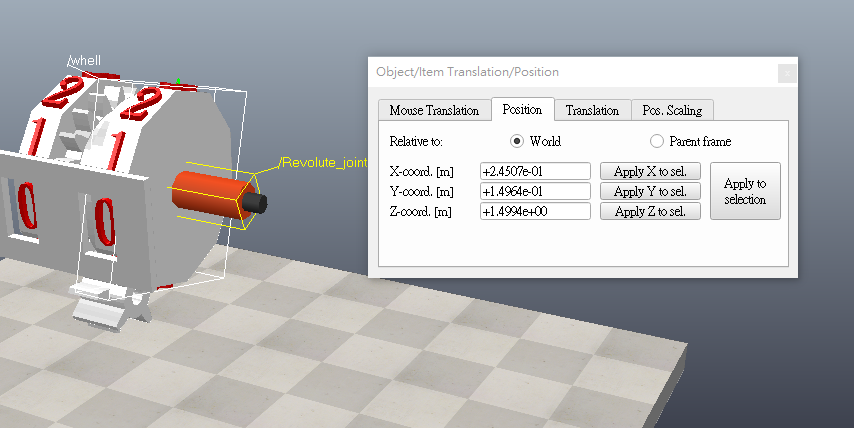
\includegraphics[width=15cm]{23}
\caption{\Large Simplified Operation diagram  簡化操作圖}\label{fig.23}
\end{center}
\end{figure}


\section{The Bill of Materials item class 物料清單項目類別 }

\fontsize{12}{2.5pt}\sectionef 
 {The Bill of Materials is a list of components necessary to build a product. In Odoo,
however, the BOM is best described by what PLM would consider the virtual representation
of the production process. That might seem counter intuitive at first considering the
previously mentioned operation item class, but in fact since the BOM is a compound item it
points directly to all item types necessary to produce the end product (Figure 24). For
example, let’s say that to build a product it is required 3 different parts and 4 different
operations; the BOM of said product would list all of them as well as specify the order in
which these are utilized.}\\[1pt]

\fontsize{12}{2.5pt}\sectionef  
{物料清單是建立產品所需組件的清單。 在奧杜,
然而,BOM 最好透過 PLM 認為的虛擬表示來描述
的生產過程。 乍一看,這似乎違反直覺
前面提到了操作項類,但實際上由於BOM是複合項它
直接指向生產最終產品所需的所有項目類型(圖 24)。 為了
例如,假設要建造一個產品,需要 3 個不同的部件和 4 個不同的部件
營運; 所述產品的 BOM 將列出所有這些產品並指定順序
這些都被利用了。}\\[15pt]

\begin{figure}[hbt!]
\begin{center}
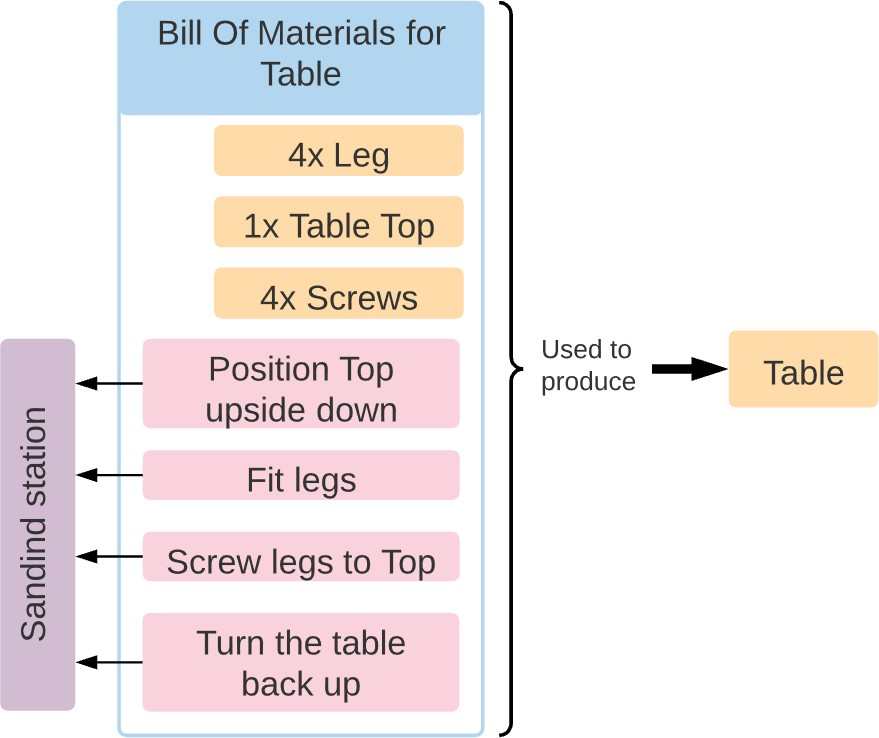
\includegraphics[width=15cm]{24}
\caption{\Large Simplified BOM diagram  簡化的 BOM 圖}\label{fig.24}
\end{center}
\end{figure}

\section{Manufacturing order item class and work order item class  製造訂單項目類和工作訂單項目類 }

\fontsize{12}{2.5pt}\sectionef 
 {Along the standard items that are considered within Odoo, orders are the ones that
represent commencement within the system. They are signaling that a change is taking place
somehow and somewhere. In the case of a manufacturing order it represents the order to
manufacture N number of specific products using it’s BOM as a base. It is as consequence
of that MO that work orders are automatically generated by Odoo (one for each necessary
operation listed in the BOM) and allocated throughout available necessary workcenters
(Figure 25). }\\[1pt]

\fontsize{12}{2.5pt}\sectionef  
{沿著 Odoo 中考慮的標準項目,訂單是那些
代表系統內的開始。 他們發出信號表明變化正在發生
以某種方式和某處。 在製造訂單的情況下,它代表訂單
使用 BOM 作為基礎製造 N 種特定產品。 其結果就是
該 MO 的工作訂單由 Odoo 自動產生(每個必要的工作訂單一個)
BOM 中列出的操作)並指派到可用的必要工作中心
(圖 25)。}\\[15pt]

\fontsize{12}{2.5pt}\sectionef 
 {The work order is the main form in which the manufacturing operators interact with Odoo,
it presents all the instructions specified by the operation item, as well as control towards its
completion. When a WO takes place the operator signals through the interface its beginning,
its completion and even any quality control check points required while the system keeps
track of timing and performance (Figure 26). Once all WO are done the MO can be declared
done and the materials and components specified in the BOM are consumed and the N copies
of the product is added to inventory. All that makes the work order a central piece as far as
MES is concerned.  }\\[1pt]

\fontsize{12}{2.5pt}\sectionef  
{工單是製造操作員與 Odoo 互動的主要形式,
它呈現了操作項指定的所有指令,以及對其的控制
完成。 當 WO 發生時,操作員透過介面發出開始訊號,
它的完成,甚至是系統保持時所需的任何品質控制檢查點
追蹤時間和性能(圖 26)。 一旦所有 WO 完成,即可宣布 MO
完成並且BOM中指定的材料和組件被消耗並且N份
產品的數量被加到庫存中。 所有這些使得工單成為核心部分
MES很在意。}\\[15pt]

\begin{figure}[hbt!]
\begin{center}
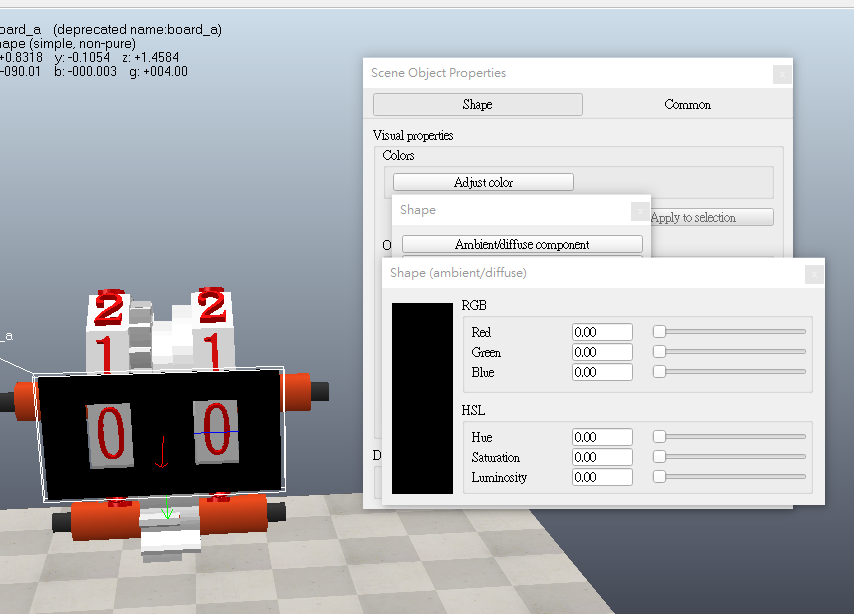
\includegraphics[width=15cm]{25}
\caption{\Large Simplified orders diagram  簡化訂單圖}\label{fig.25}
\end{center}
\end{figure}

\begin{figure}[hbt!]
\begin{center}
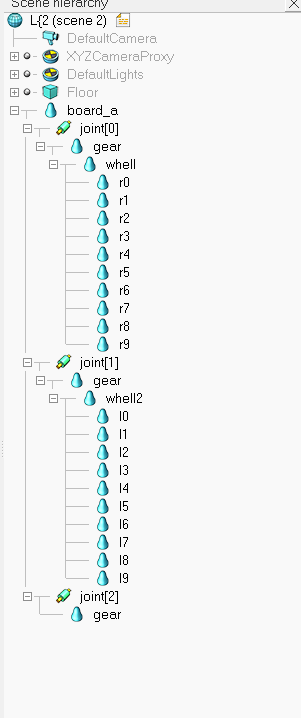
\includegraphics[width=15cm]{26}
\caption{\Large Operator interface during the WO  WO 期間的操作員介面}\label{fig.26}
\end{center}
\end{figure}


\section{ The engineering change order 工程變更單 }

\fontsize{12}{2.5pt}\sectionef 
 {As explained in the beginning of chapter 2 the Odoo management software considers
PLM mainly as a tool for tracking change and improvements. Its application module is
external to the normal flow of manufacturing but acts as an expansion to it. Its focal item
class is the Engineering Change Order (ECO). }\\[1pt]

\fontsize{12}{2.5pt}\sectionef  
{如第 2 章開頭所解釋的,Odoo 管理軟體考慮
PLM 主要作為追蹤變更和改進的工具。 其應用模組為
位於正常製造流程之外,但充當其擴展。 其重點項目
類別是工程變更單(ECO)。}\\[15pt]



\fontsize{12}{2.5pt}\sectionef 
 {An ECO is an item class that outlines the proposed changes to the product or the parts that
would be affected by the change. In other words, is a central information hub for everyone
associated with a given product. }\\[1pt]

\fontsize{12}{2.5pt}\sectionef  
{ECO 是一個項目類別,概述了產品或零件的建議變更
將受到該變化的影響。 換句話說,就是每個人的中央資訊中心
與給定產品相關聯。}\\[15pt]


\fontsize{12}{2.5pt}\sectionef 
 {The idea is to signal the need for change to a product item or a BOM item, hold the files
that are relevant to the change and apply the change or at least signal that the change has been
implemented, all while keeping the history of al the previous changes. All very useful in the
future and serve as a process to streamline product development and help improve
products/production.}\\[1pt]

\fontsize{12}{2.5pt}\sectionef  
{這個想法是表明需要更改產品項目或 BOM 項目,保存文件
與變更相關並應用變更或至少表示變更已經
實施,同時保留所有先前更改的歷史記錄。 一切都非常有用
未來並作為簡化產品開發並幫助改進的流程
產品/生產。}\\[15pt]



\begin{figure}[hbt!]
\begin{center}
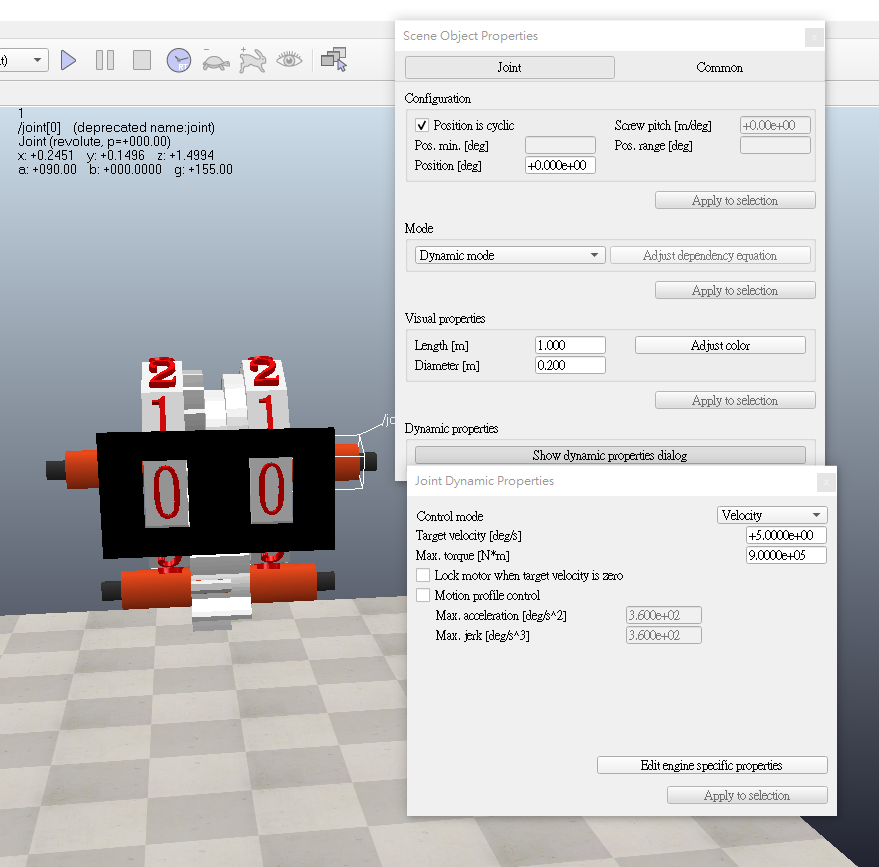
\includegraphics[width=15cm]{27}
\caption{\Large Simplified ECO function diagram 簡化的ECO功能圖}\label{fig.27}
\end{center}
\end{figure}